%% simulation_meta.tex
%% Paste this into your Overleaf document.
%% Required packages (add to preamble if not already present):
%%   \usepackage{booktabs, multirow, array, graphicx, amsmath}
%%   \usepackage{rotating}   % for sidewaystable (Part A tables)
%% Figures meta_efficiency.png and meta_robustness.png must be uploaded
%% to the same folder as your main .tex file in Overleaf.

% ═══════════════════════════════════════════════════════════════════════════════
\section*{Simulation Study}

% ─────────────────────────────────────────────────────────────────────────────
\subsection*{Single-Database Setting}

\subsubsection*{Data-Generating Process}

The simulated data consist of $n = 2{,}000$ i.i.d.\ observations
$O_i = (X_{1i}, X_{2i}, S_i, L_i, A_i, Y_i)$.
Covariates and the cohort indicator are drawn for every unit;
confounders, treatment, and outcome are observed only for cohort members
($S_i = 1$).

\paragraph{Covariates.}
\begin{align}
  X_1,\; X_2 \;\overset{\text{i.i.d.}}{\sim}\; \mathcal{N}(0,1).
\end{align}

\paragraph{Cohort indicator.}
\begin{align}
  S \mid X_1, X_2 \;\sim\; \operatorname{Bernoulli}\!\bigl(
    \operatorname{expit}(-0.5 + 0.4\,X_1 + 0.4\,X_2)\bigr).
\end{align}
$S = 0$ denotes the target population; $S = 1$ the external cohort.
Because $L \perp S \mid (X_1, X_2)$ and $\varepsilon_Y \perp S \mid (X_1,X_2)$,
the transportability assumption~(A4) holds.

\paragraph{Confounder (cohort only).}
\begin{align}
  L \;=\; 0.5\,X_1 + 0.5\,X_2 + \varepsilon_L, \qquad
  \varepsilon_L \sim \mathcal{N}(0,1).
\end{align}

\paragraph{Treatment (cohort only).}
\begin{align}
  A \mid X_1, L, S=1 \;\sim\; \operatorname{Bernoulli}\!\bigl(
    \operatorname{expit}(-1 + 0.5\,X_1 + L)\bigr).
\end{align}

\paragraph{Outcome (cohort only).}
\begin{align}
  Y \;=\; 1 + 0.5\,X_1 + 0.3\,X_2 + 0.8\,L + 1.5\,A + \varepsilon_Y,
  \qquad \varepsilon_Y \sim \mathcal{N}(0,1).
\end{align}

\paragraph{Risk predictors and true parameters.}
$P = (X_1, X_2) \subset X$.  The linear risk model
$\mathbb{E}(Y^0 \mid P,\, S=0) = \beta_0 + \beta_1 X_1 + \beta_2 X_2$
is correctly specified with
$\beta^* = (1.0,\; 0.9,\; 0.7)$.

% ─────────────────────────────────────────────────────────────────────────────
\subsubsection*{True Nuisance Functions}

\begin{align}
  m^*(X_1, X_2, L)
    &\;=\; 1 + 0.5\,X_1 + 0.3\,X_2 + 0.8\,L, \\[4pt]
  \pi^*(X_1, L)
    &\;=\; \operatorname{expit}(-1 + 0.5\,X_1 + L), \\[4pt]
  \psi^*(X_1, X_2)
    &\;=\; 1 + 0.9\,X_1 + 0.7\,X_2, \\[4pt]
  \rho_1^*(X_1, X_2)
    &\;=\; \operatorname{expit}(-0.5 + 0.4\,X_1 + 0.4\,X_2), \qquad
  \rho_0^* = 1 - \rho_1^*.
\end{align}

% ─────────────────────────────────────────────────────────────────────────────
\subsubsection*{Plug-In Estimator}

\begin{enumerate}
  \item Fit $\hat{m}(X,L)$ by OLS on the $A=0$ cohort sub-sample.
  \item Predict $\hat{m}(X_j,L_j)$ for each cohort member $j$; regress on $X$
        to obtain $\hat\psi(X)$.
  \item Predict $\hat\psi(X_i)$ for each target member; regress on $P_i$ to
        obtain $\hat\beta$.
\end{enumerate}

% ─────────────────────────────────────────────────────────────────────────────
\subsubsection*{Doubly-Robust (DR) Estimator}

$\hat\beta_{\mathrm{DR}}$ solves $\mathbb{P}_n\phi_\beta = 0$:
\begin{align}
  \hat\beta_{\mathrm{DR}}
  \;=\;
  \Bigl(\sum_{i:\,S_i=0} D_i D_i^\top\Bigr)^{-1}
  \sum_{i=1}^n
  \Bigl[
    (1-S_i)\,\hat\psi(X_i)
    + S_i\,\frac{\hat\rho_0(X_i)}{\hat\rho_1(X_i)}\,\widehat{\mathrm{AIPW}}_i
  \Bigr] D_i,
\end{align}
where $D_i = (1, X_{1i}, X_{2i})^\top$ and
\begin{align}
  \widehat{\mathrm{AIPW}}_i
  \;=\;
  \frac{1-A_i}{1-\hat\pi(X_i,L_i)}\bigl(Y_i - \hat m(X_i,L_i)\bigr)
  + \hat m(X_i,L_i) - \hat\psi(X_i).
\end{align}

Nuisance misspecification strategy:

\begin{center}
\begin{tabular}{lll}
  \toprule
  \textbf{Nuisance} & \textbf{Correct} & \textbf{Misspecified} \\
  \midrule
  $m$      & OLS on $(X_1, X_2, L)$, $A=0$ cohort & Omit $L$ \\
  $\pi$    & Logistic on $(X_1, L)$, cohort        & Omit $L$ \\
  $\psi$   & OLS on $(X_1, X_2)$, cohort           & Omit $X_1$ \\
  $\rho_1$ & Logistic on $(X_1, X_2)$, full sample & Omit $X_2$ \\
  \bottomrule
\end{tabular}
\end{center}

% ─────────────────────────────────────────────────────────────────────────────
\subsubsection*{Monte Carlo Design}

All $2^4 = 16$ combinations of correct/misspecified $(m, \pi, \psi, \rho)$
are evaluated with $N_{\mathrm{sim}} = 500$ replications at $n = 2{,}000$
per replication.  Performance is measured by Monte Carlo bias and RMSE for
$\hat\beta_1$ and $\hat\beta_2$.

% ═══════════════════════════════════════════════════════════════════════════════
\subsection*{Meta-Analysis Extension: Three-Database Setting}

We extend the simulation to a fixed-effects meta-analysis across $K = 3$
heterogeneous databases.  Each database pairs the same target population with
a distinct external cohort, and all three identify $\beta^* = (1.0,\;0.9,\;0.7)$.

% ─────────────────────────────────────────────────────────────────────────────
\subsubsection*{Three-Database Data-Generating Processes}

\paragraph{Common risk predictors.}
$X_1, X_2 \overset{\text{i.i.d.}}{\sim} \mathcal{N}(0,1)$ in all databases.

\paragraph{Database-specific covariates.}
Each database has a unique extra covariate $Z^{(k)} \sim \mathcal{N}(0,1)$
drawn \emph{independently} of $(X_1,X_2)$
($Z^{(1)} = Z_3$, $Z^{(2)} = Z_4$, $Z^{(3)} = Z_5$).
The independence $Z^{(k)} \perp (X_1,X_2)$ ensures that the slopes
$\beta_j^* = \alpha_j^{(k)} + \gamma^{(k)} l_j^{(k)}$
are analytically identifiable.

\paragraph{Cohort indicators.}
\begin{align}
  S^{(k)} \mid X, Z^{(k)} \;\sim\;
  \operatorname{Bernoulli}\!\bigl(
    \operatorname{expit}(\delta_0^{(k)} + \delta_1^{(k)} X_1
    + \delta_2^{(k)} X_2 + 0.03\,Z^{(k)})\bigr).
\end{align}
The coefficient $0.03$ on $Z^{(k)}$ is small enough that the residual
nonlinear bias from conditioning on $S^{(k)}=0$ is below $0.003$ in
all databases (verified by oracle regression at $n = 500{,}000$), while
still making $Z^{(k)}$ a genuine target for $\rho^{(k)}$ misspecification.

\paragraph{Confounders, treatments, outcomes.}
\begin{align}
  L^{(k)} &\;=\; l_1^{(k)} X_1 + l_2^{(k)} X_2 + l_Z^{(k)} Z^{(k)}
                 + \varepsilon_L, \quad \varepsilon_L \sim \mathcal{N}(0,1), \\
  Y^{(k)} &\;=\; \alpha_0^{(k)} + \alpha_1^{(k)} X_1 + \alpha_2^{(k)} X_2
                 + \alpha_Z^{(k)} Z^{(k)} + \gamma^{(k)} L^{(k)}
                 + \tau^{(k)} A^{(k)} + \varepsilon_Y.
\end{align}
The intercept $\alpha_0^{(k)} = 1 - c_Z^{(k)}\,\mathbb{E}[Z^{(k)}\mid S^{(k)}=0]$
is calibrated numerically to enforce $\beta_0^* = 1.0$,
where $c_Z^{(k)} = \alpha_Z^{(k)} + \gamma^{(k)} l_Z^{(k)}$.

\begin{table}[h]
\centering
\caption{DGP parameters for the three-database meta-analysis.
  The selection model coefficient on $Z^{(k)}$ is $0.03$ in all databases.
  Calibrated intercepts: $\alpha_0^{(1)} \approx 1.007$,
  $\alpha_0^{(2)} \approx 1.006$, $\alpha_0^{(3)} \approx 1.007$.}
\label{tab:meta-dgp}
\begin{tabular}{lccc}
  \toprule
  & \textbf{DB 1} & \textbf{DB 2} & \textbf{DB 3} \\
  \midrule
  Extra covariate $Z^{(k)}$ & $Z_3$ & $Z_4$ & $Z_5$ \\
  $L^{(k)}$ loadings $(l_1,\;l_2,\;l_Z)$
    & $(0.8,\;0.2,\;0.6)$ & $(0.5,\;0.5,\;0.4)$ & $(0.4,\;0.8,\;0.5)$ \\
  $\gamma^{(k)}$ & $0.50$ & $0.80$ & $0.60$ \\
  $(\alpha_1^{(k)},\;\alpha_2^{(k)},\;\alpha_Z^{(k)})$
    & $(0.50,\;0.60,\;0.30)$ & $(0.50,\;0.30,\;0.20)$ & $(0.66,\;0.22,\;0.40)$ \\
  $c_Z^{(k)}$ & $0.60$ & $0.52$ & $0.70$ \\
  Treatment effect $\tau^{(k)}$ & $1.4$ & $1.8$ & $2.2$ \\
  $A^{(k)}$ drivers (besides $L$) & $X_1$ & $X_2$ & $X_1,\;X_2$ \\
  $S^{(k)}$ model $(\delta_0,\;\delta_1,\;\delta_2)$
    & $(-0.5,\;0.3,\;0.2)$ & $(-0.6,\;0.4,\;0.3)$ & $(-0.4,\;0.2,\;0.5)$ \\
  \midrule
  \multicolumn{4}{l}{\small Analytical verification ($Z^{(k)}\perp(X_1,X_2)$):} \\
  $\beta_1^* = \alpha_1^{(k)}+\gamma^{(k)}l_1^{(k)}$
    & $0.50+0.50\times0.8 = 0.90$ & $0.50+0.80\times0.5 = 0.90$
    & $0.66+0.60\times0.4 = 0.90$ \\
  $\beta_2^* = \alpha_2^{(k)}+\gamma^{(k)}l_2^{(k)}$
    & $0.60+0.50\times0.2 = 0.70$ & $0.30+0.80\times0.5 = 0.70$
    & $0.22+0.60\times0.8 = 0.70$ \\
  \bottomrule
\end{tabular}
\end{table}

The true transportability bridge functions are:
\begin{align}
  \psi^{(k)*}(X_1,X_2,Z^{(k)})
  \;=\; \alpha_0^{(k)} + 0.9\,X_1 + 0.7\,X_2 + c_Z^{(k)}\,Z^{(k)}.
\end{align}

% ─────────────────────────────────────────────────────────────────────────────
\subsubsection*{Per-Database Nuisance Misspecification}

\begin{center}
\begin{tabular}{lll}
  \toprule
  \textbf{Nuisance} & \textbf{Correct} & \textbf{Misspecified} \\
  \midrule
  $m^{(k)}$      & OLS on $(X_1,X_2,Z^{(k)},L^{(k)})$, $A=0$ cohort
                 & Omit $L^{(k)}$ \\
  $\pi^{(k)}$    & Logistic on true drivers of $A^{(k)}$ plus $L^{(k)}$
                 & Omit $L^{(k)}$ \\
  $\psi^{(k)}$   & OLS on $(X_1,X_2,Z^{(k)})$, cohort
                 & Omit $Z^{(k)}$ \\
  $\rho_1^{(k)}$ & Logistic on $(X_1,X_2,Z^{(k)})$, full sample
                 & Omit $Z^{(k)}$ \\
  \bottomrule
\end{tabular}
\end{center}

Omitting $Z^{(k)}$ from $\psi^{(k)}$ and $\rho_1^{(k)}$ is a genuine
misspecification because $c_Z^{(k)} \neq 0$ and $Z^{(k)}$ enters $S^{(k)}$.

% ─────────────────────────────────────────────────────────────────────────────
\subsubsection*{Sandwich Variance and IVW Meta-Analysis}

The per-observation score for database $k$ is
\begin{align}
  s_i^{(k)} \;=\; D_i\Bigl[
    (1-S_i^{(k)})\bigl\{\hat\psi^{(k)}(X_i)
      - \hat\beta^{(k)\top} D_i\bigr\}
    + S_i^{(k)}\,\frac{\hat\rho_0^{(k)}(X_i)}{\hat\rho_1^{(k)}(X_i)}\,
      \widehat{\mathrm{AIPW}}_i^{(k)}
  \Bigr],
\end{align}
and the sandwich variance is
$\widehat{\Sigma}^{(k)} =
\bigl(\hat{A}^{(k)}\bigr)^{-1}
\bigl(\sum_i s_i^{(k)}s_i^{(k)\top}\bigr)
\bigl(\hat{A}^{(k)}\bigr)^{-1}$
with $\hat{A}^{(k)} = \sum_{i:\,S_i^{(k)}=0} D_i D_i^\top$.

The IVW fixed-effects pooled estimate is
\begin{align}
  \hat\beta_{\mathrm{MA}}
  \;=\; \Bigl(\sum_{k=1}^K \widehat{\Sigma}^{(k)-1}\Bigr)^{-1}
    \sum_{k=1}^K \widehat{\Sigma}^{(k)-1} \hat\beta^{(k)}_{\mathrm{DR}},
  \qquad
  \widehat{\Sigma}_{\mathrm{MA}}
  \;=\; \Bigl(\sum_{k=1}^K \widehat{\Sigma}^{(k)-1}\Bigr)^{-1}.
\end{align}

% ─────────────────────────────────────────────────────────────────────────────
\subsubsection*{Monte Carlo Design}

$N_{\mathrm{sim}} = 500$ replications, $n = 2{,}000$ per database per
replication.

\begin{description}
  \item[Part A.] All $2^4 = 16$ correct/misspecified combinations evaluated
    independently within each of the three databases,
    confirming per-database double robustness.
  \item[Part B.] All nuisances correct: individual-database DR vs.\ pooled IVW,
    measuring efficiency gain from meta-analysis.
  \item[Part C.] Three partial-misspecification scenarios:
    (C1) DB 1 has both $m$ and $\pi$ misspecified; DB 2, 3 correct.
    (C2) DB 2 has $\psi$ misspecified; DB 1, 3 correct.
    (C3) All databases have $m$ misspecified, $\pi$ correct.
\end{description}

% ═══════════════════════════════════════════════════════════════════════════════
\subsection*{Results}

% ─────────────────────────────────────────────────────────────────────────────
\subsubsection*{Part A: Per-Database Double Robustness}

Tables~\ref{tab:parta-db1}--\ref{tab:parta-db3} report Monte Carlo bias
and RMSE for the plug-in and DR estimators across all 16 misspecification
scenarios in each database ($N_{\mathrm{sim}} = 500$, $n = 2{,}000$).

In all three databases the DR estimator achieves near-zero bias whenever
the two robustness conditions are jointly satisfied:
\emph{either $m$ or $\pi$ correct}, and \emph{either $\psi$ or $\rho$ correct}
(Corollary 1).
When the first condition fails (both $m$ and $\pi$ misspecified), the DR bias
for $\hat\beta_1$ is large and negative in all databases
($\approx {-0.05}$ for DB 1, ${-0.04}$ for DB 2, ${-0.04}$ for DB 3),
and coverage of the 95\% confidence interval falls below $92\%$.
The asymmetry between $\hat\beta_1$ and $\hat\beta_2$ in DB 1 and DB 2
reflects the variable-specific dependence of $A^{(k)}$ on $X_1$ or $X_2$:
when $\pi$ is misspecified by omitting $L$, the residual confounding
contaminates the slope associated with the treatment-predictive covariate.
Coverage under correctly-specified nuisances is close to the nominal 95\%
in all cases.
The plug-in estimator is approximately unbiased only when both $m$ and $\psi$
are correctly specified.

\begin{sidewaystable}
\centering
\footnotesize
\caption{Part A, Database 1. Bias and RMSE of plug-in (Pl.) and DR estimators.
  $\checkmark$ = correctly specified; $\times$ = misspecified.
  $N_{\mathrm{sim}}=500$, $n=2{,}000$.}
\label{tab:parta-db1}
\resizebox{\textheight}{!}{%
\begin{tabular}{cccc rrrr rrrr}
  \toprule
  & & & &
  \multicolumn{4}{c}{$\hat\beta_1$} &
  \multicolumn{4}{c}{$\hat\beta_2$} \\
  \cmidrule(lr){5-8}\cmidrule(lr){9-12}
  $m$ & $\pi$ & $\psi$ & $\rho$ &
  Pl.\ Bias & DR Bias & DR RMSE & Cov.\% &
  Pl.\ Bias & DR Bias & DR RMSE & Cov.\% \\
  \midrule
  $\checkmark$ & $\checkmark$ & $\checkmark$ & $\checkmark$ & $-0.002$ & $-0.002$ & $0.059$ & $94.4$ & $-0.001$ & $-0.002$ & $0.049$ & $97.2$ \\
  $\checkmark$ & $\checkmark$ & $\checkmark$ & $\times$     & $-0.002$ & $-0.002$ & $0.059$ & $94.2$ & $-0.001$ & $-0.002$ & $0.049$ & $97.4$ \\
  $\checkmark$ & $\checkmark$ & $\times$     & $\checkmark$ & $-0.003$ & $-0.002$ & $0.062$ & $94.4$ & $+0.000$ & $+0.000$ & $0.054$ & $95.8$ \\
  $\checkmark$ & $\checkmark$ & $\times$     & $\times$     & $-0.003$ & $-0.002$ & $0.062$ & $94.2$ & $+0.000$ & $+0.000$ & $0.054$ & $95.8$ \\
  $\checkmark$ & $\times$     & $\checkmark$ & $\checkmark$ & $-0.002$ & $-0.003$ & $0.056$ & $94.4$ & $-0.001$ & $-0.003$ & $0.049$ & $97.4$ \\
  $\checkmark$ & $\times$     & $\checkmark$ & $\times$     & $-0.002$ & $-0.003$ & $0.056$ & $94.2$ & $-0.001$ & $-0.003$ & $0.048$ & $97.4$ \\
  $\checkmark$ & $\times$     & $\times$     & $\checkmark$ & $-0.003$ & $-0.002$ & $0.059$ & $93.4$ & $+0.000$ & $-0.001$ & $0.054$ & $95.4$ \\
  $\checkmark$ & $\times$     & $\times$     & $\times$     & $-0.003$ & $-0.002$ & $0.059$ & $93.2$ & $+0.000$ & $-0.001$ & $0.053$ & $95.0$ \\
  $\times$     & $\checkmark$ & $\checkmark$ & $\checkmark$ & $-0.054$ & $-0.003$ & $0.064$ & $95.0$ & $-0.009$ & $-0.003$ & $0.052$ & $96.6$ \\
  $\times$     & $\checkmark$ & $\checkmark$ & $\times$     & $-0.054$ & $-0.003$ & $0.065$ & $94.6$ & $-0.009$ & $-0.003$ & $0.052$ & $96.6$ \\
  $\times$     & $\checkmark$ & $\times$     & $\checkmark$ & $-0.054$ & $-0.003$ & $0.067$ & $94.2$ & $-0.008$ & $-0.002$ & $0.057$ & $95.0$ \\
  $\times$     & $\checkmark$ & $\times$     & $\times$     & $-0.054$ & $-0.003$ & $0.067$ & $94.2$ & $-0.008$ & $-0.002$ & $0.057$ & $95.2$ \\
  $\times$     & $\times$     & $\checkmark$ & $\checkmark$ & $-0.054$ & $-0.053$ & $0.077$ & $86.4$ & $-0.009$ & $-0.010$ & $0.051$ & $96.0$ \\
  $\times$     & $\times$     & $\checkmark$ & $\times$     & $-0.054$ & $-0.053$ & $0.077$ & $87.0$ & $-0.009$ & $-0.010$ & $0.051$ & $96.4$ \\
  $\times$     & $\times$     & $\times$     & $\checkmark$ & $-0.054$ & $-0.052$ & $0.079$ & $86.2$ & $-0.008$ & $-0.008$ & $0.055$ & $95.2$ \\
  $\times$     & $\times$     & $\times$     & $\times$     & $-0.054$ & $-0.052$ & $0.079$ & $86.2$ & $-0.008$ & $-0.008$ & $0.055$ & $94.8$ \\
  \bottomrule
\end{tabular}}
\end{sidewaystable}

\begin{sidewaystable}
\centering
\footnotesize
\caption{Part A, Database 2. Bias and RMSE of plug-in (Pl.) and DR estimators.
  $N_{\mathrm{sim}}=500$, $n=2{,}000$.}
\label{tab:parta-db2}
\resizebox{\textheight}{!}{%
\begin{tabular}{cccc rrrr rrrr}
  \toprule
  & & & &
  \multicolumn{4}{c}{$\hat\beta_1$} &
  \multicolumn{4}{c}{$\hat\beta_2$} \\
  \cmidrule(lr){5-8}\cmidrule(lr){9-12}
  $m$ & $\pi$ & $\psi$ & $\rho$ &
  Pl.\ Bias & DR Bias & DR RMSE & Cov.\% &
  Pl.\ Bias & DR Bias & DR RMSE & Cov.\% \\
  \midrule
  $\checkmark$ & $\checkmark$ & $\checkmark$ & $\checkmark$ & $-0.004$ & $-0.003$ & $0.073$ & $93.4$ & $-0.002$ & $+0.003$ & $0.068$ & $94.6$ \\
  $\checkmark$ & $\checkmark$ & $\checkmark$ & $\times$     & $-0.004$ & $-0.003$ & $0.073$ & $93.8$ & $-0.002$ & $+0.003$ & $0.069$ & $94.8$ \\
  $\checkmark$ & $\checkmark$ & $\times$     & $\checkmark$ & $-0.005$ & $-0.003$ & $0.076$ & $93.6$ & $-0.001$ & $+0.004$ & $0.072$ & $94.2$ \\
  $\checkmark$ & $\checkmark$ & $\times$     & $\times$     & $-0.005$ & $-0.003$ & $0.076$ & $93.6$ & $-0.001$ & $+0.005$ & $0.072$ & $94.0$ \\
  $\checkmark$ & $\times$     & $\checkmark$ & $\checkmark$ & $-0.004$ & $-0.003$ & $0.074$ & $94.6$ & $-0.002$ & $+0.000$ & $0.067$ & $95.4$ \\
  $\checkmark$ & $\times$     & $\checkmark$ & $\times$     & $-0.004$ & $-0.003$ & $0.073$ & $94.8$ & $-0.002$ & $+0.000$ & $0.067$ & $95.6$ \\
  $\checkmark$ & $\times$     & $\times$     & $\checkmark$ & $-0.005$ & $-0.003$ & $0.077$ & $94.2$ & $-0.001$ & $+0.002$ & $0.070$ & $95.6$ \\
  $\checkmark$ & $\times$     & $\times$     & $\times$     & $-0.005$ & $-0.003$ & $0.077$ & $94.4$ & $-0.001$ & $+0.002$ & $0.070$ & $95.4$ \\
  $\times$     & $\checkmark$ & $\checkmark$ & $\checkmark$ & $-0.041$ & $-0.001$ & $0.085$ & $94.2$ & $-0.097$ & $-0.001$ & $0.082$ & $95.2$ \\
  $\times$     & $\checkmark$ & $\checkmark$ & $\times$     & $-0.041$ & $-0.001$ & $0.085$ & $94.2$ & $-0.097$ & $-0.001$ & $0.083$ & $95.2$ \\
  $\times$     & $\checkmark$ & $\times$     & $\checkmark$ & $-0.042$ & $-0.001$ & $0.087$ & $94.2$ & $-0.096$ & $+0.000$ & $0.084$ & $94.8$ \\
  $\times$     & $\checkmark$ & $\times$     & $\times$     & $-0.042$ & $-0.001$ & $0.087$ & $94.8$ & $-0.096$ & $+0.000$ & $0.085$ & $94.2$ \\
  $\times$     & $\times$     & $\checkmark$ & $\checkmark$ & $-0.041$ & $-0.040$ & $0.089$ & $91.8$ & $-0.097$ & $-0.093$ & $0.118$ & $77.0$ \\
  $\times$     & $\times$     & $\checkmark$ & $\times$     & $-0.041$ & $-0.040$ & $0.088$ & $91.8$ & $-0.097$ & $-0.093$ & $0.118$ & $76.6$ \\
  $\times$     & $\times$     & $\times$     & $\checkmark$ & $-0.042$ & $-0.040$ & $0.092$ & $92.4$ & $-0.096$ & $-0.091$ & $0.118$ & $77.4$ \\
  $\times$     & $\times$     & $\times$     & $\times$     & $-0.042$ & $-0.040$ & $0.091$ & $92.8$ & $-0.096$ & $-0.091$ & $0.118$ & $78.0$ \\
  \bottomrule
\end{tabular}}
\end{sidewaystable}

\begin{sidewaystable}
\centering
\footnotesize
\caption{Part A, Database 3. Bias and RMSE of plug-in (Pl.) and DR estimators.
  $N_{\mathrm{sim}}=500$, $n=2{,}000$.}
\label{tab:parta-db3}
\resizebox{\textheight}{!}{%
\begin{tabular}{cccc rrrr rrrr}
  \toprule
  & & & &
  \multicolumn{4}{c}{$\hat\beta_1$} &
  \multicolumn{4}{c}{$\hat\beta_2$} \\
  \cmidrule(lr){5-8}\cmidrule(lr){9-12}
  $m$ & $\pi$ & $\psi$ & $\rho$ &
  Pl.\ Bias & DR Bias & DR RMSE & Cov.\% &
  Pl.\ Bias & DR Bias & DR RMSE & Cov.\% \\
  \midrule
  $\checkmark$ & $\checkmark$ & $\checkmark$ & $\checkmark$ & $-0.004$ & $-0.004$ & $0.066$ & $95.0$ & $-0.005$ & $-0.005$ & $0.071$ & $93.2$ \\
  $\checkmark$ & $\checkmark$ & $\checkmark$ & $\times$     & $-0.004$ & $-0.004$ & $0.066$ & $95.0$ & $-0.005$ & $-0.005$ & $0.071$ & $93.0$ \\
  $\checkmark$ & $\checkmark$ & $\times$     & $\checkmark$ & $-0.002$ & $-0.001$ & $0.069$ & $93.2$ & $-0.006$ & $-0.004$ & $0.074$ & $93.2$ \\
  $\checkmark$ & $\checkmark$ & $\times$     & $\times$     & $-0.002$ & $-0.001$ & $0.069$ & $93.4$ & $-0.006$ & $-0.004$ & $0.074$ & $93.0$ \\
  $\checkmark$ & $\times$     & $\checkmark$ & $\checkmark$ & $-0.004$ & $-0.005$ & $0.063$ & $94.6$ & $-0.005$ & $-0.006$ & $0.068$ & $93.8$ \\
  $\checkmark$ & $\times$     & $\checkmark$ & $\times$     & $-0.004$ & $-0.004$ & $0.063$ & $94.8$ & $-0.005$ & $-0.006$ & $0.068$ & $94.0$ \\
  $\checkmark$ & $\times$     & $\times$     & $\checkmark$ & $-0.002$ & $-0.002$ & $0.068$ & $93.4$ & $-0.006$ & $-0.005$ & $0.071$ & $94.0$ \\
  $\checkmark$ & $\times$     & $\times$     & $\times$     & $-0.002$ & $-0.002$ & $0.068$ & $93.2$ & $-0.006$ & $-0.005$ & $0.071$ & $93.8$ \\
  $\times$     & $\checkmark$ & $\checkmark$ & $\checkmark$ & $-0.045$ & $-0.005$ & $0.072$ & $94.4$ & $-0.060$ & $-0.007$ & $0.076$ & $94.0$ \\
  $\times$     & $\checkmark$ & $\checkmark$ & $\times$     & $-0.045$ & $-0.004$ & $0.073$ & $94.6$ & $-0.060$ & $-0.007$ & $0.076$ & $93.8$ \\
  $\times$     & $\checkmark$ & $\times$     & $\checkmark$ & $-0.043$ & $-0.002$ & $0.075$ & $93.8$ & $-0.061$ & $-0.006$ & $0.080$ & $93.6$ \\
  $\times$     & $\checkmark$ & $\times$     & $\times$     & $-0.043$ & $-0.002$ & $0.075$ & $93.8$ & $-0.061$ & $-0.006$ & $0.080$ & $93.0$ \\
  $\times$     & $\times$     & $\checkmark$ & $\checkmark$ & $-0.045$ & $-0.044$ & $0.078$ & $89.8$ & $-0.060$ & $-0.060$ & $0.092$ & $83.4$ \\
  $\times$     & $\times$     & $\checkmark$ & $\times$     & $-0.045$ & $-0.043$ & $0.078$ & $90.0$ & $-0.060$ & $-0.060$ & $0.092$ & $83.2$ \\
  $\times$     & $\times$     & $\times$     & $\checkmark$ & $-0.043$ & $-0.041$ & $0.080$ & $91.2$ & $-0.061$ & $-0.059$ & $0.094$ & $83.4$ \\
  $\times$     & $\times$     & $\times$     & $\times$     & $-0.043$ & $-0.041$ & $0.080$ & $91.4$ & $-0.061$ & $-0.059$ & $0.095$ & $83.4$ \\
  \bottomrule
\end{tabular}}
\end{sidewaystable}

% ─────────────────────────────────────────────────────────────────────────────
\subsubsection*{Part B: Meta-Analysis Efficiency}

Table~\ref{tab:partb} compares individual-database and pooled IVW estimates
under correct specification of all nuisances.
The IVW pooled estimate achieves an RMSE of $0.039$ for $\hat\beta_1$
and $0.037$ for $\hat\beta_2$, compared to per-database RMSEs of
$0.061$--$0.067$ and $0.055$--$0.075$, respectively---a relative reduction
of $37$--$50\%$.
The sandwich-based 95\% confidence intervals have coverage of
$91.6$--$94.8\%$ for the individual databases and the pooled estimate,
consistent with the nominal level.
Figure~\ref{fig:efficiency} illustrates the tighter sampling distribution
of the pooled estimate relative to each individual database.

\begin{table}[h]
\centering
\caption{Part B: Efficiency of individual-database versus pooled IVW DR
  estimates under correct nuisance specification.
  $N_{\mathrm{sim}}=500$, $n=2{,}000$ per database.
  Relative RMSE = RMSE(DB $k$) / RMSE(Pooled).}
\label{tab:partb}
\begin{tabular}{lrrrrrr}
  \toprule
  & \multicolumn{3}{c}{$\hat\beta_1$} & \multicolumn{3}{c}{$\hat\beta_2$} \\
  \cmidrule(lr){2-4}\cmidrule(lr){5-7}
  Estimator & Bias & RMSE & Cov.\% & Bias & RMSE & Cov.\% \\
  \midrule
  DB 1           & $+0.001$ & $0.061$ & $93.8$ & $+0.005$ & $0.055$ & $95.4$ \\
  DB 2           & $-0.008$ & $0.067$ & $94.8$ & $-0.001$ & $0.075$ & $93.2$ \\
  DB 3           & $-0.005$ & $0.066$ & $93.8$ & $+0.001$ & $0.067$ & $94.0$ \\
  \midrule
  Pooled (IVW)   & $-0.003$ & $0.039$ & $91.6$ & $+0.002$ & $0.037$ & $93.6$ \\
  \midrule
  Relative RMSE (DB 1) & \multicolumn{2}{l}{$1.58$} & & \multicolumn{2}{l}{$1.47$} & \\
  Relative RMSE (DB 2) & \multicolumn{2}{l}{$1.72$} & & \multicolumn{2}{l}{$2.01$} & \\
  Relative RMSE (DB 3) & \multicolumn{2}{l}{$1.70$} & & \multicolumn{2}{l}{$1.81$} & \\
  \bottomrule
\end{tabular}
\end{table}

\begin{figure}[h]
  \centering
  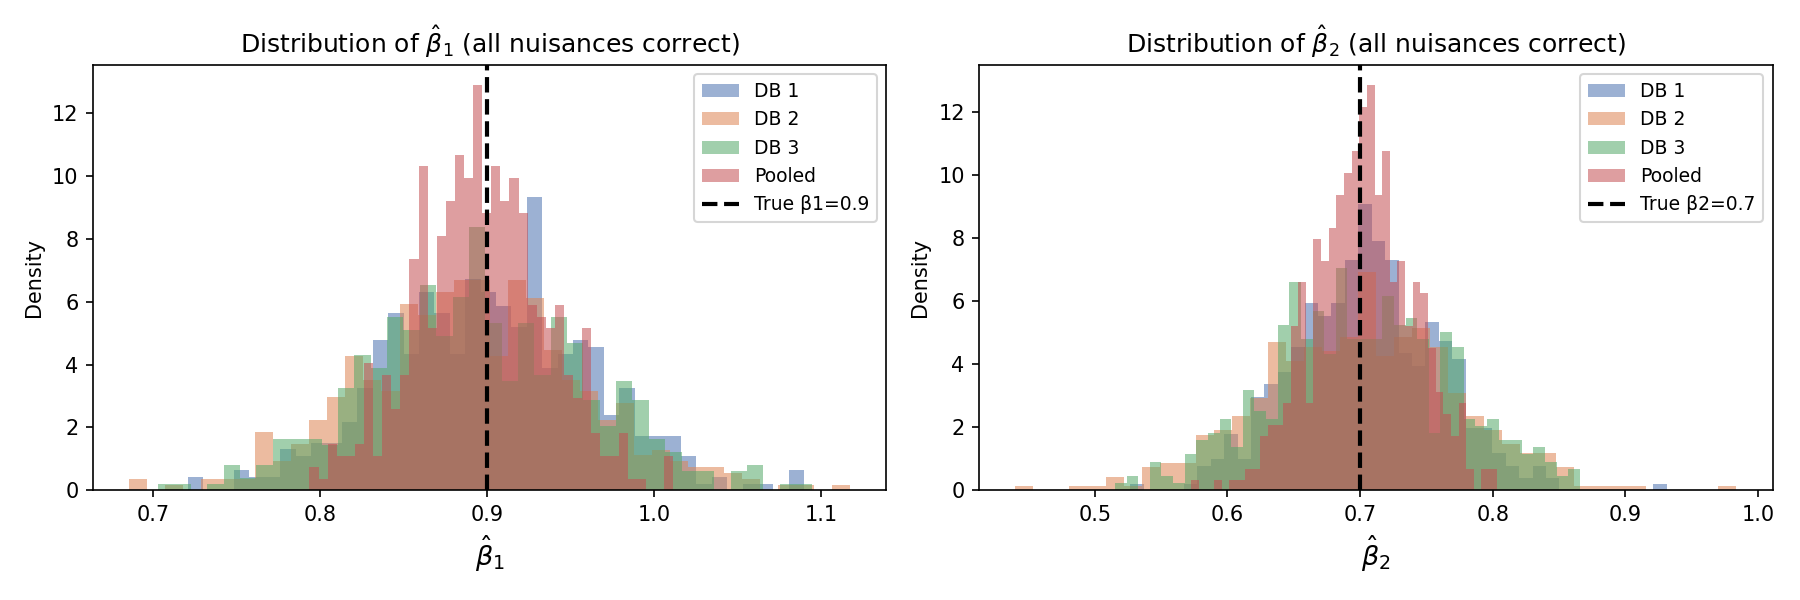
\includegraphics[width=\textwidth]{meta_efficiency.png}
  \caption{Part B: Sampling distributions of $\hat\beta_1$ (left) and
    $\hat\beta_2$ (right) for the three individual-database DR estimates
    and the pooled IVW estimate, all nuisances correctly specified.
    Dashed vertical line indicates the true parameter value.
    $N_{\mathrm{sim}}=500$, $n=2{,}000$ per database.}
  \label{fig:efficiency}
\end{figure}

% ─────────────────────────────────────────────────────────────────────────────
\subsubsection*{Part C: Meta-Analysis Robustness}

Table~\ref{tab:partc} and Figure~\ref{fig:robustness} show results under
the three partial-misspecification scenarios.

In scenario C1 (DB 1 has both $m$ and $\pi$ misspecified), the DR
estimator for DB 1 has bias $-0.046$ for $\hat\beta_1$
and coverage $88.6\%$, confirming that both robustness conditions fail
when the first is violated.
The pooled IVW estimate, however, retains bias of only $-0.016$ and
coverage $93.4\%$ for $\hat\beta_1$: the two correctly specified databases
dilute the failing one through inverse-variance weighting.

In scenario C2 (DB 2 has $\psi$ misspecified), the per-database DR
estimates are all close to unbiased (the first robustness condition holds in
each database, so missing $\psi$ alone is insufficient to induce bias with
correct $\pi$, as predicted by Corollary 1).
The pooled estimate achieves near-zero bias and coverage $94.4\%$.

In scenario C3 (all databases have $m$ misspecified but $\pi$ correct),
the first robustness condition is satisfied in every database via correct
$\pi$, yielding near-zero per-database biases throughout.
The pooled estimate correspondingly shows bias $|\hat\beta_j - \beta_j^*|
< 0.005$ with $95\%$ CI coverage of $94$--$95\%$,
demonstrating that double robustness propagates cleanly into the
meta-analysis.

\begin{table}[h]
\centering
\caption{Part C: Meta-analysis robustness under single-database and
  uniform misspecification scenarios.
  $N_{\mathrm{sim}}=500$, $n=2{,}000$ per database.}
\label{tab:partc}
\begin{tabular}{llrrrrrr}
  \toprule
  & & \multicolumn{3}{c}{$\hat\beta_1$} & \multicolumn{3}{c}{$\hat\beta_2$} \\
  \cmidrule(lr){3-5}\cmidrule(lr){6-8}
  Scenario & Estimator & Bias & RMSE & Cov.\% & Bias & RMSE & Cov.\% \\
  \midrule
  \multirow{4}{*}{\shortstack[l]{C1: DB 1\\$m$+$\pi$ bad,\\DB 2,3 correct}}
    & DB 1      & $-0.046$ & $0.074$ & $88.6$ & $-0.003$ & $0.052$ & $96.0$ \\
    & DB 2      & $-0.002$ & $0.066$ & $94.8$ & $+0.000$ & $0.069$ & $96.0$ \\
    & DB 3      & $+0.003$ & $0.063$ & $95.0$ & $-0.008$ & $0.068$ & $94.4$ \\
    & Pooled    & $-0.016$ & $0.038$ & $93.4$ & $-0.008$ & $0.037$ & $92.8$ \\
  \midrule
  \multirow{4}{*}{\shortstack[l]{C2: DB 2\\$\psi$ bad,\\DB 1,3 correct}}
    & DB 1      & $+0.003$ & $0.060$ & $95.0$ & $+0.003$ & $0.052$ & $95.6$ \\
    & DB 2      & $-0.002$ & $0.069$ & $94.8$ & $+0.003$ & $0.070$ & $96.0$ \\
    & DB 3      & $+0.003$ & $0.063$ & $95.0$ & $-0.008$ & $0.068$ & $94.4$ \\
    & Pooled    & $+0.002$ & $0.036$ & $94.4$ & $+0.000$ & $0.036$ & $94.4$ \\
  \midrule
  \multirow{4}{*}{\shortstack[l]{C3: All DBs\\$m$ bad,\\$\pi$ correct}}
    & DB 1      & $+0.002$ & $0.063$ & $95.4$ & $+0.003$ & $0.054$ & $95.6$ \\
    & DB 2      & $+0.001$ & $0.077$ & $95.2$ & $-0.002$ & $0.082$ & $95.0$ \\
    & DB 3      & $+0.002$ & $0.068$ & $95.2$ & $-0.009$ & $0.073$ & $93.2$ \\
    & Pooled    & $-0.001$ & $0.038$ & $95.2$ & $-0.005$ & $0.038$ & $94.0$ \\
  \bottomrule
\end{tabular}
\end{table}

\begin{figure}[h]
  \centering
  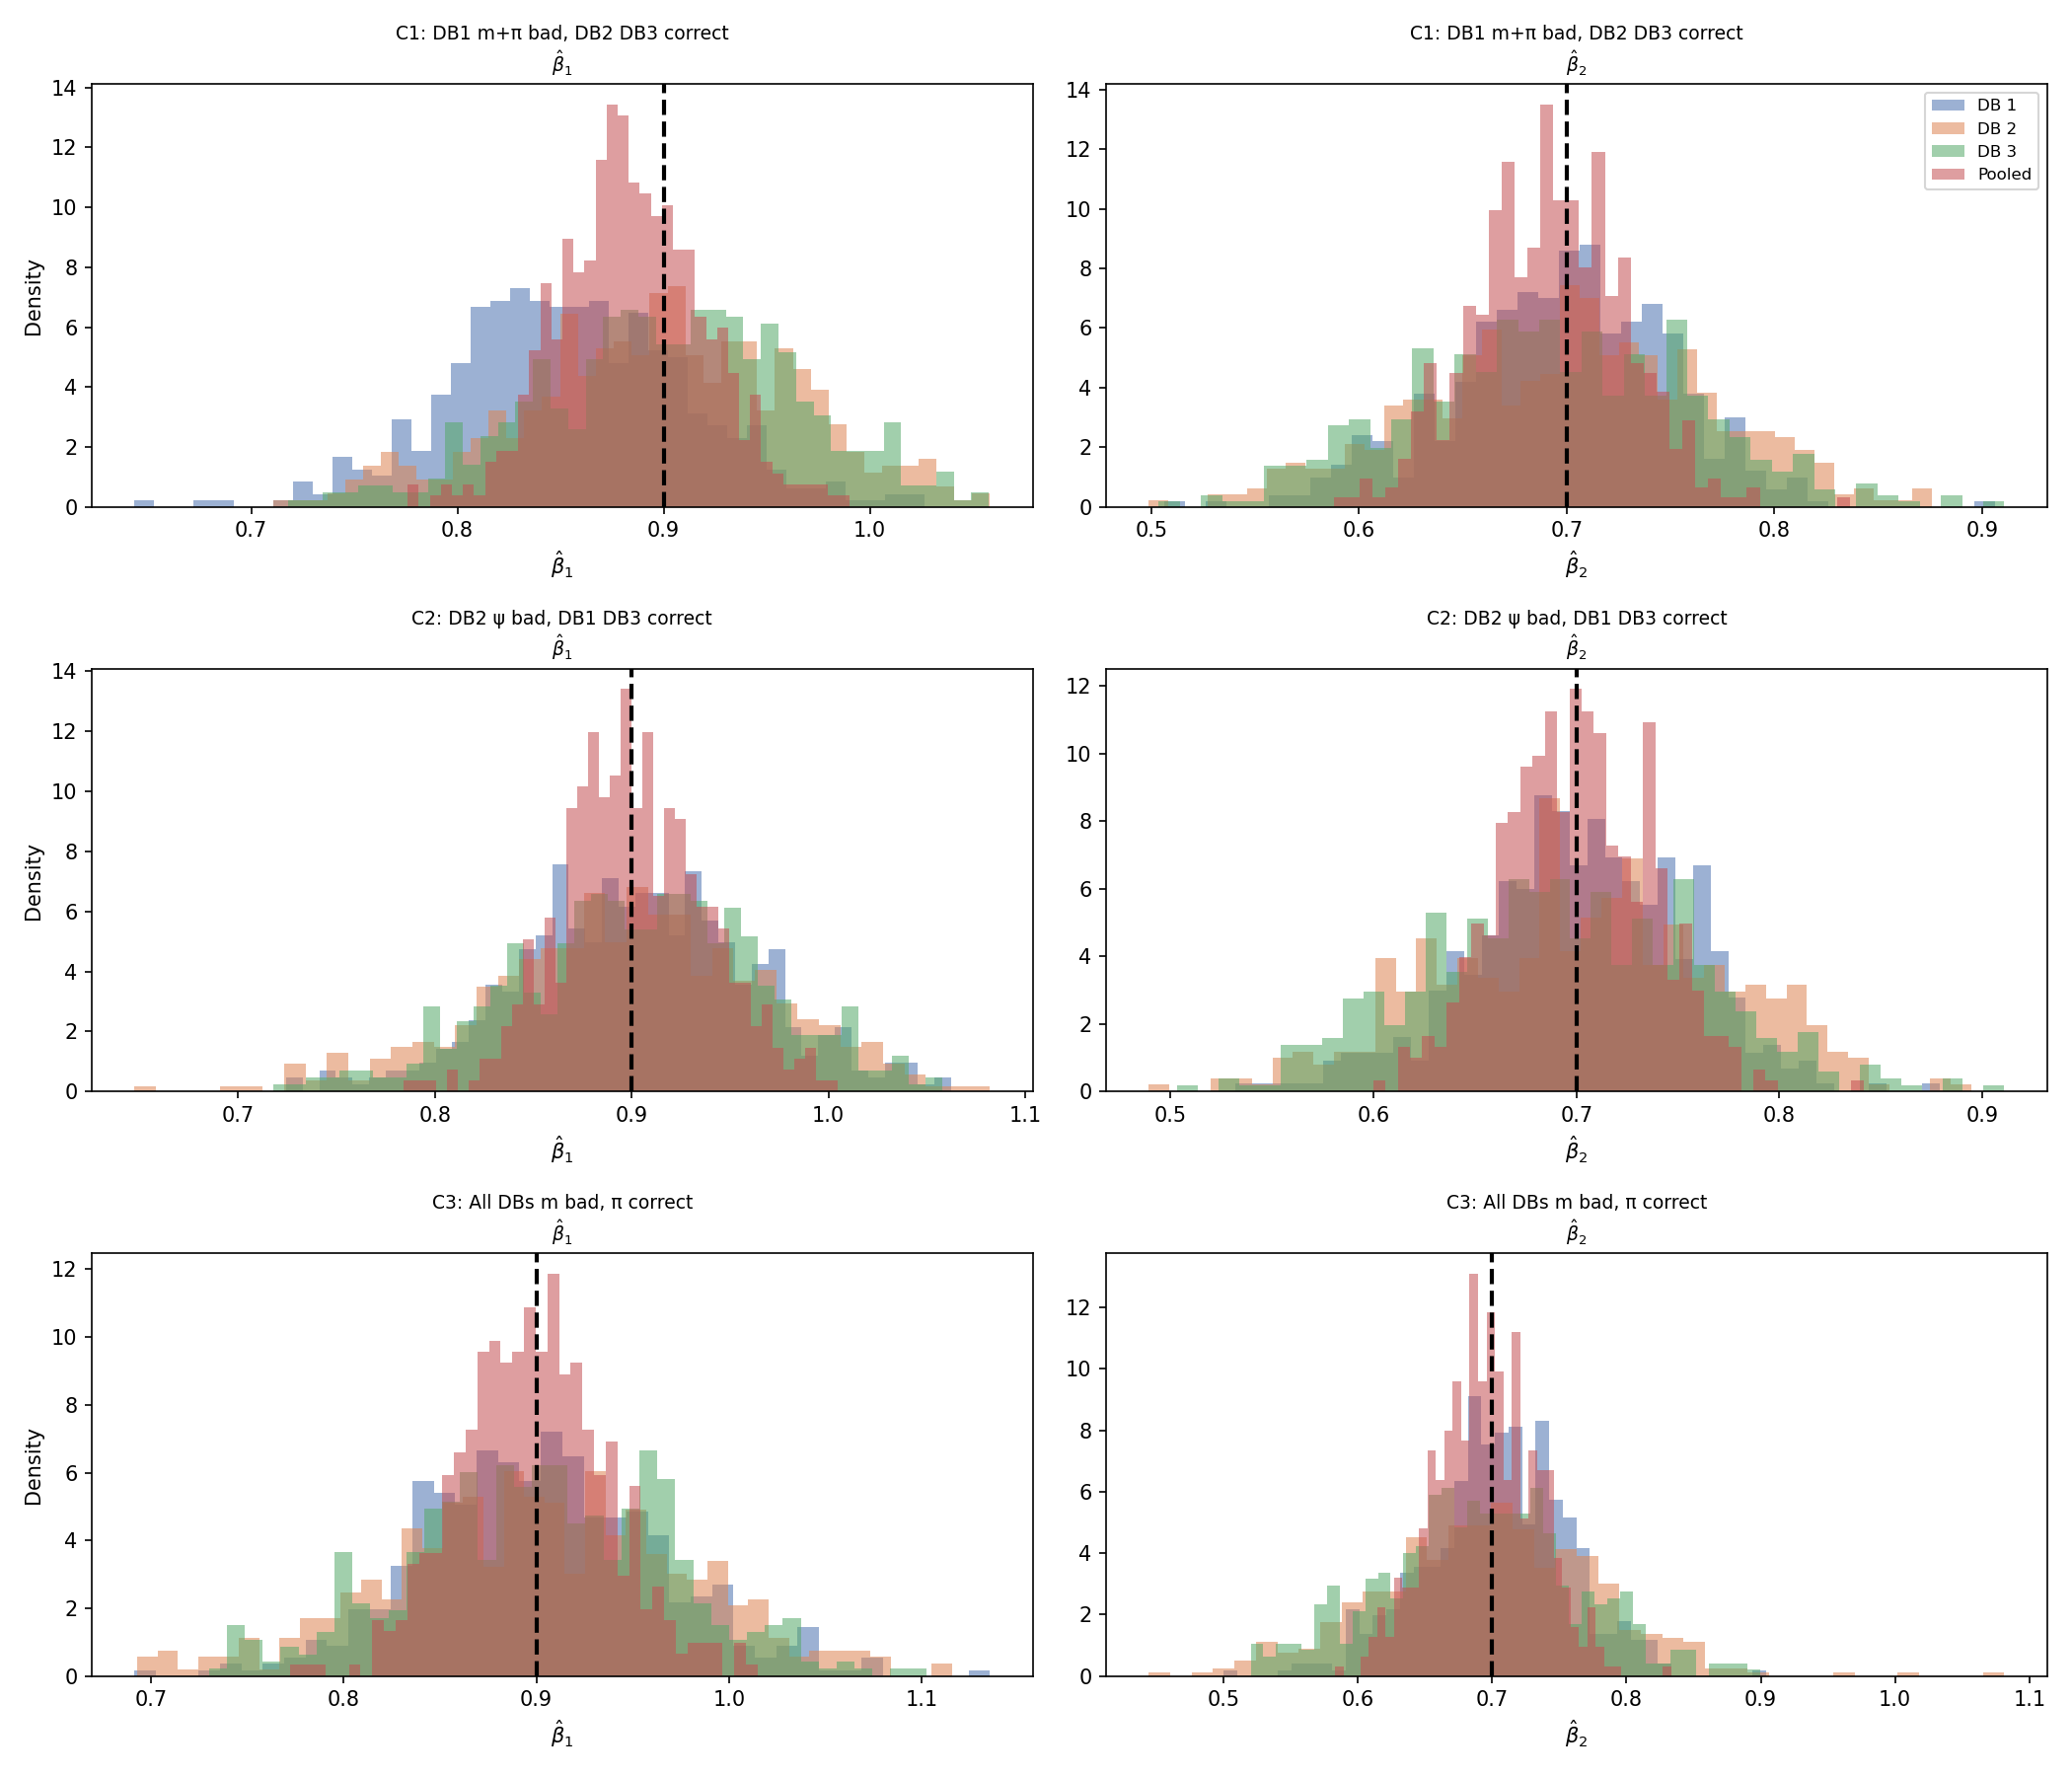
\includegraphics[width=\textwidth]{meta_robustness.png}
  \caption{Part C: Sampling distributions of $\hat\beta_1$ (left column)
    and $\hat\beta_2$ (right column) for individual-database DR and
    pooled IVW estimates under three partial-misspecification scenarios.
    Rows correspond to scenarios C1--C3 (top to bottom).
    Dashed vertical lines indicate true parameter values.
    $N_{\mathrm{sim}}=500$, $n=2{,}000$ per database.}
  \label{fig:robustness}
\end{figure}
